\begin{figure}
\scriptsize{
\medskip
%%%%%%%%%%%%%%%%%%%%
$
\inferrule
{
}
{\jp \FH{\phi}{\skipstmt}{\phi}}
\;(\textsc{Skip})
$
\medskip
%%%%%%%%%%%%%%%%%%%%
$
\inferrule
{
P \not \in \dom(\refines)
}
{\jp \FH{\phi}{\assert{\locExpr}}{\phi}}
\;(\textsc{Assert1})
$
\medskip
%%%%%%%%%%%%%%%%%%%%
$
\inferrule
{
}
{\jp \FH{\phi \wedge \locExpr}{\assert{\locExpr}}{\phi}}
\;(\textsc{Assert2})
$
\medskip
%%%%%%%%%%%%%%%%%%%%
$
\inferrule
{
}
{\jp \FH{e}{\yield{e}}{e}}
\;(\textsc{Yield})
$
\medskip
%%%%%%%%%%%%%%%%%%%%
$
\inferrule
{
\actions(A) = (\rho, \alpha, m) \\ \phi_1 \Rightarrow \rho \\ \phi_1 \wedge \alpha \Rightarrow \phi_2
}
{\jp \FH{\phi_1}{\call{A}}{\phi_2}}
\;(\textsc{Atomic})
$
\medskip
%%%%%%%%%%%%%%%%%%%%
$
\inferrule
{
\specs(P) = (\phi, \psi) \\ H \neq \{\}
}
{\jp \FH{\phi}{\call{P}}{\psi}}
\;(\textsc{Proc1})
$
\medskip
%%%%%%%%%%%%%%%%%%%%
$
\inferrule
{
\specs(P) = (\phi, \psi) \\ P \in \dom(\refines) \\ \jp \FH{\phi}{\call{\refines(P)}}{\psi}
}
{\jp \FH{\phi}{\call{P}}{\psi}}
\;(\textsc{Proc2})
$
\medskip
%%%%%%%%%%%%%%%%%%%%
$
\inferrule
{
\specs(P) = (\phi, \psi)
}
{\jp \FH{\rho \wedge \phi}{\async{P}}{\rho}}
\;(\textsc{Async})
$
\medskip
%%%%%%%%%%%%%%%%%%%%
$
\inferrule
{
\jp \FH{\phi_1 \wedge e}{s}{\phi_2}
}
{\jp \FH{\phi_1 \wedge e}{\ablock{e}{s}}{\phi_2}}
\;(\textsc{Ablock})
$
\medskip
%%%%%%%%%%%%%%%%%%%%
$
\inferrule
{
\jp \FH{\phi_1}{s_1}{\phi_2} \\ \jp \FH{\phi_2}{s_2}{\phi_3}
}
{\jp \FH{\phi_1}{s_1;s_2}{\phi_3}}
\;(\textsc{Seq})
$
\medskip
%%%%%%%%%%%%%%%%%%%%
$
\inferrule
{
\jp \FH{e \wedge \phi_1}{s_1}{\phi_2} \\ \jp \FH{\neg e \wedge \phi_1}{s_2}{\phi_2}
}
{\jp \FH{\phi_1}{\ite{\locExpr}{s_1}{s_2}}{\phi_2}}
\;(\textsc{Ite})
$
\medskip
%%%%%%%%%%%%%%%%%%%%
$
\inferrule
{
\jp \FH{e \wedge \locExpr}{s}{e}
}
{\jp \FH{e}{\while{e}{\locExpr}{s}}{e \wedge \neg \locExpr}}
\;(\textsc{While})
$
\medskip
%%%%%%%%%%%%%%%%%%%%

}
\caption{Sequential rules for partial correctness}
\label{fig:sequential-correctness}
\end{figure}

{\bf Non-interference.}
Let $\Yield$ be the set of yield predicates, $\Pre$ be the set of preconditions,
and $\Post$ be the set of postconditions, and $\Ablock$ be the set of atomic blocks in the entire program.
Let $\FV \subseteq \VarName \setminus \Var$ be a set of fresh variables and $\Lambda$ be a one-one 
substitution function from $\ThreadLocals \cup \Locals$ to $\FV$.
Let $\Lambda(\phi)$ represent the result of applying $\Lambda$ to the expression $\phi$.
For each predicate $\phi \in \Yield \cup \Pre \cup \Post$
and for each atomic block $\ablock{e}{s} \in \Ablock$, we prove the following judgment:
\[
\jp \FH{\Lambda(\phi) \wedge e}{s}{\Lambda(\phi)}
\]

Let $\Yield'$ be the set of yield predicates anywhere in the program except in the bodies of procedures
in  $\dom(\refines)$.
Let ${\cal P}$ be the set of procedures called from anywhere in the program except from the bodies of 
procedures in $\dom(\refines)$.
Let $\Pre'$ be the set of preconditions and $\Post'$ be the set of postconditions of the procedures in ${\cal P}$.
For each predicate $\phi \in \Yield' \cup \Pre' \cup \Post'$ and for each $P \in \dom(\refines) \cap {\cal P}$ such that
$\actions(P) = (\rho, \alpha, m)$, prove the following valid:
\[
\Lambda(\phi) \circ \rho \circ \alpha \Rightarrow \Lambda(\phi)
\]

{\bf Commutativity.}
Let $\FV_1,\FV_2 \subseteq \VarName \setminus \Var$ be two sets of disjoint fresh variables.
Let $\Lambda_1$ and $\Lambda_2$ be one-one 
substitution functions from $\ThreadLocals \cup \Locals$ to $\FV_1$ and $\FV_2$ respectively.
For all $A_1,A_2 \in \ActionName$ such that $\actions(A_1) = (\rho_1,\alpha_1,m_1)$ and $\actions(A_2) = (\rho_2,\alpha_2,m_2)$,
if $m_1 \in \{B,R\}$ or $m_2 \in \{B,L\}$ then prove the following valid:
\[
\begin{array}{l}
(\Lambda_1(\rho_1) \wedge \Lambda_2(\rho_2)) \circ (\Lambda_1(\alpha_1) \wedge \Same(\FV_2)) \circ (\Lambda_1(\alpha_2) \wedge \Same(\FV_1)) \\ 
\Rightarrow (\Lambda_1(\alpha_2) \wedge \Same(\FV_1)) \circ (\Lambda_1(\alpha_1) \wedge \Same(\FV_2))
\end{array}
\]
For all $A_1,A_2 \in \ActionName$ such that $\actions(A_1) = (\rho_1,\alpha_1,m_1)$ and $\actions(A_2) = (\rho_2,\alpha_2,m_2)$,
if $m_1 \in \{B,R\}$ then prove the following unsatisfiable:
\[
\Lambda_1(\rho_1) \circ (\Lambda_2(\rho_2) \circ \Lambda_2(\alpha_2)) \circ \neg \Lambda_1(\rho_1)
\]
For all $A_1,A_2 \in \ActionName$ such that $\actions(A_1) = (\rho_1,\alpha_1,m_1)$ and $\actions(A_2) = (\rho_2,\alpha_2,m_2)$,
if $m_1 \in \{B,L\}$ then prove the following unsatisfiable:
\[
\neg \Lambda_1(\rho_1) \circ (\Lambda_2(\rho_2) \circ \Lambda_2(\alpha_2)) \circ \Lambda_1(\rho_1)
\]

\begin{figure}
\scriptsize{
\medskip
%%%%%%%%%%%%%%%%%%%%
$
\inferrule
{
}
{P \vdash \skipstmt : \epsilon}
\;(\textsc{Skip})
$
\medskip
%%%%%%%%%%%%%%%%%%%%
$
\inferrule
{
}
{P \vdash \assert{\locExpr} : \epsilon}
\;(\textsc{Assert})
$
\medskip
%%%%%%%%%%%%%%%%%%%%
$
\inferrule
{
}
{P \vdash \yield{e} : \epsilon}
\;(\textsc{Yield})
$
\medskip
%%%%%%%%%%%%%%%%%%%%
$
\inferrule
{
\mov(P') \neq \perp \\ \act(P') \Rightarrow \havoc{H}
}
{P \vdash \call{P'} : \epsilon}
\;(\textsc{Call-Loop})
$
\medskip
%%%%%%%%%%%%%%%%%%%%
$
\inferrule
{
\mov(P') \neq \perp \\ \act(P') \Rightarrow \act{P}
}
{P \vdash \ablock{e}{s} : A}
\;(\textsc{Call-Action})
$
\medskip
%%%%%%%%%%%%%%%%%%%%
$
\inferrule
{
\mov(P') \neq \perp \\ \act(P') \Rightarrow \havoc{H}
}
{P \vdash \async{P'} : \epsilon}
\;(\textsc{Async})
$
\medskip
%%%%%%%%%%%%%%%%%%%%
$
\inferrule
{
\jp \FH{e}{s}{\havoc{H \cup L}}
}
{P \vdash \ablock{e}{s} : \epsilon}
\;(\textsc{Ablock-Loop})
$
\medskip
%%%%%%%%%%%%%%%%%%%%
$
\inferrule
{
\jp \FH{e}{s}{\act(P)}
}
{P \vdash \ablock{e}{s} : A}
\;(\textsc{Ablock-Action})
$
\medskip
%%%%%%%%%%%%%%%%%%%%
$
\inferrule
{
P \vdash s_1 : \re_1 \\ P \vdash s_2 : \re_2
}
{P \vdash s_1;s_2 : \re_1\cdot\re_2}
\;(\textsc{Seq})
$
\medskip
%%%%%%%%%%%%%%%%%%%%
$
\inferrule
{
P \vdash s_1 : \re_1 \\ P \vdash s_2 : \re_2
}
{P \vdash \ite{\locExpr}{s_1}{s_2} : \re_1+\re_2}
\;(\textsc{Ite})
$
\medskip
%%%%%%%%%%%%%%%%%%%%
$
\inferrule
{
P \vdash s : \re
}
{P \vdash \while{e}{\locExpr}{s} : \re^*}
\;(\textsc{While})
$
\medskip
%%%%%%%%%%%%%%%%%%%%

}
\caption{Refinement rules}
\label{fig:refinement}
\end{figure}


\begin{figure}
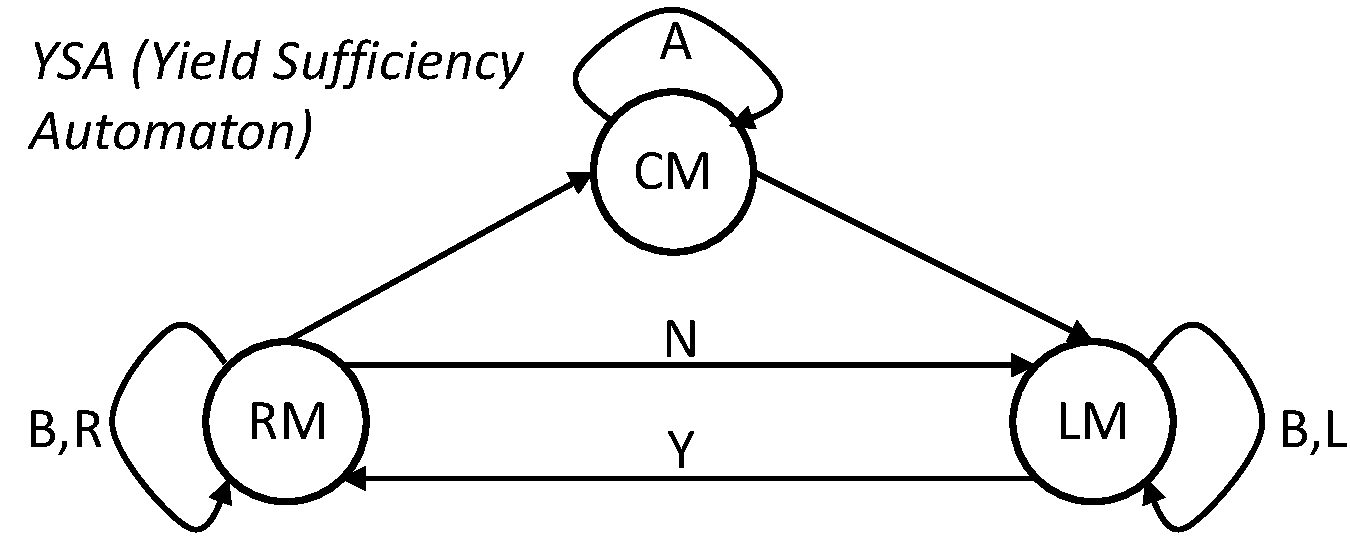
\includegraphics[scale=0.35]{YieldTypeCheckingAutomaton.pdf}
\caption{Specification for yield sufficiency}
\label{fig:YieldTypeCheckingAutomaton}
\end{figure}

\begin{figure}
\scriptsize{
\medskip
%%%%%%%%%%%%%%%%%%%%
$
\inferrule
{
}
{P \vdash \skipstmt : x \leadsto x}
\;(\textsc{Skip})
$
\medskip
%%%%%%%%%%%%%%%%%%%%
$
\inferrule
{
}
{P \vdash \assert{\locExpr} : x \leadsto x}
\;(\textsc{Assert})
$
\medskip
%%%%%%%%%%%%%%%%%%%%
$
\inferrule
{
}
{P \vdash \yield{e} : x \leadsto \RM}
\;(\textsc{Yield})
$
\medskip
%%%%%%%%%%%%%%%%%%%%
$
\inferrule
{
\mov(P') = B
}
{P \vdash \call{P'} : x \leadsto x}
\;(\textsc{CallBothMover})
$
\medskip
%%%%%%%%%%%%%%%%%%%%
$
\inferrule
{
\mov(P') = R
}
{P \vdash \call{P'} : \RM \leadsto \RM}
\;(\textsc{CallRightMover})
$
\medskip
%%%%%%%%%%%%%%%%%%%%
$
\inferrule
{
\mov(P') = L
}
{P \vdash \call{P'} : x \leadsto \LM}
\;(\textsc{CallLeftMover})
$
\medskip
%%%%%%%%%%%%%%%%%%%%
$
\inferrule
{
\mov(P') = N
}
{P \vdash \call{P'} : \RM \leadsto \LM}
\;(\textsc{CallYield})
$
\medskip
%%%%%%%%%%%%%%%%%%%%
$
\inferrule
{
\mov(P') = \perp
}
{P \vdash \call{P'} : x \leadsto \RM}
\;(\textsc{CallYield})
$
\medskip
%%%%%%%%%%%%%%%%%%%%
$
\inferrule
{
}
{P \vdash \async{P'} : x \leadsto \LM}
\;(\textsc{Async})
$
\medskip
%%%%%%%%%%%%%%%%%%%%
$
\inferrule
{
x \in \{\RM,\CM\}
}
{P \vdash \ablock{e}{s} : x \leadsto \CM}
\;(\textsc{Ablock})
$
\medskip
%%%%%%%%%%%%%%%%%%%%
$
\inferrule
{
P \vdash s_1 : x \leadsto y \\ P \vdash s_2 : y \leadsto z
}
{P \vdash s_1;s_2 : x \leadsto z}
\;(\textsc{Seq})
$
\medskip
%%%%%%%%%%%%%%%%%%%%
$
\inferrule
{
P \vdash s_1 : x \leadsto y \\ P \vdash s_2 : x \leadsto y
}
{P \vdash \ite{\locExpr}{s_1}{s_2} : x \leadsto y}
\;(\textsc{Ite})
$
\medskip
%%%%%%%%%%%%%%%%%%%%
$
\inferrule
{
P \vdash s : x \leadsto x
}
{P \vdash \while{e}{\locExpr}{s} : x \leadsto x}
\;(\textsc{While})
$
\medskip
%%%%%%%%%%%%%%%%%%%%

}
\caption{Yield sufficiency rules}
\label{fig:yield-sufficiency}
\end{figure}

\subsection{Responsiveness}

\newcommand{\stutter}{\skipstmt}

\[
\inferrule
{
\jp \FH{e \wedge \locExpr}{s}{e} \\ e \wedge \locExpr \Rightarrow m \geq 0 \\ \jr s \preceq \beta \\ e \wedge \locExpr \wedge \beta \Rightarrow m' < m \\ \neg \locExpr \wedge \stutter \Rightarrow \alpha \\ \beta \circ \alpha \Rightarrow \alpha 
}
{\jp \FH{e}{\twhile{e}{m,\alpha}{\locExpr}{s}}{e \wedge \neg \locExpr}}
\;(\textsc{While})
\]


\begin{figure}
\scriptsize{
\medskip
%%%%%%%%%%%%%%%%%%%%
$
\inferrule
{
}
{\jr \skipstmt \preceq \stutter}
\;(\textsc{Skip})
$
\medskip
%%%%%%%%%%%%%%%%%%%%
$
\inferrule
{
}
{\jr \assert{\locExpr} \preceq \stutter}
\;(\textsc{Assert})
$
\medskip
%%%%%%%%%%%%%%%%%%%%
$
\inferrule
{
}
{\jr \yield{e} \preceq \false}
\;(\textsc{Yield})
$
\medskip
%%%%%%%%%%%%%%%%%%%%
$
\inferrule
{
\actions(A) = (\rho, \alpha, m) 
}
{\jr \call{A} \preceq \alpha}
\;(\textsc{Atomic})
$
\medskip
%%%%%%%%%%%%%%%%%%%%
$
\inferrule
{
}
{\jr \call{P} \preceq \false}
\;(\textsc{Call})
$
\medskip
%%%%%%%%%%%%%%%%%%%%
$
\inferrule
{
}
{\jr \async{P} \preceq \stutter}
\;(\textsc{Async})
$
\medskip
%%%%%%%%%%%%%%%%%%%%
$
\inferrule
{
\jr s \preceq \alpha
}
{\jr \ablock{e}{s} \preceq \alpha}
\;(\textsc{Ablock})
$
\medskip
%%%%%%%%%%%%%%%%%%%%
$
\inferrule
{
\jr s_1 \preceq \alpha_1 \\ \jr s_2 \preceq \alpha_2
}
{\jr s_1;s_2 \preceq \alpha_1 \circ \alpha_2}
\;(\textsc{Seq})
$
\medskip
%%%%%%%%%%%%%%%%%%%%
$
\inferrule
{
\jr s_1 \preceq \alpha_1 \\ \jr s_2 \preceq \alpha_2
}
{\jr \ite{\locExpr}{s_1}{s_2} \preceq (\locExpr \Rightarrow \alpha_1) \wedge (\neg \locExpr \Rightarrow \alpha_2)}
\;(\textsc{Ite})
$
\medskip
%%%%%%%%%%%%%%%%%%%%
$
\inferrule
{
}
{\jr \twhile{e}{m,\alpha}{\locExpr}{s} \preceq e \circ \alpha \circ \neg \locExpr}
\;(\textsc{While})
$
\medskip
%%%%%%%%%%%%%%%%%%%%

}
\caption{Sequential rules for responsiveness}
\label{fig:termination-correctness}
\end{figure}


\newcommand{\RefinementAny}{r}
\newcommand{\RefinementInside}{\mathrm{r^+}}
\newcommand{\RefinementOutside}{\mathrm{r^-}}

\newcommand{\ABlockAny}{a}
\newcommand{\ABlockInside}{\mathrm{a^+}}
\newcommand{\ABlockOutside}{\mathrm{a^-}}

\newcommand{\ProcLins}{\mathit{ls}}

\begin{figure}
$\ProcLins \in (\ActionName \cup \ProcName) \rightarrow (2^{\Var}, 2^{\Var})$ \\
$\ABlockAny \in \mathit{InsideABlock} ::= \ABlockInside \mid \ABlockOutside$ \\
$\RefinementAny \in \mathit{InsideRefinement} ::= \RefinementInside \mid \RefinementOutside$ \\
\\
\scriptsize{
\medskip
%%%%%%%%%%%%%%%%%%%%
$
\inferrule
{
}
{
\lins;\RefinementAny;\ABlockAny \vdash \skipstmt : \lins
}
\;(\textsc{Skip})
$
\medskip
%%%%%%%%%%%%%%%%%%%%
$
\inferrule
{
}
{
\lins;\RefinementAny;\ABlockOutside \vdash \assert{\locExpr} : \lins
}
\;(\textsc{Assert1})
$
\medskip
%%%%%%%%%%%%%%%%%%%%
$
\inferrule
{
}
{
\lins;\RefinementAny;\ABlockOutside \vdash \yield{e} : \lins
}
\;(\textsc{Yield})
$
\medskip
%%%%%%%%%%%%%%%%%%%%
$
\inferrule
{
\ProcLins(A) = (\lins,\lins') \\
\lins_L \subseteq \Locals
}
{
\lins_L,\lins;\RefinementAny;\ABlockInside \vdash \call{A} : \lins_L,\lins'
}
\;(\textsc{Atomic})
$
\medskip
%%%%%%%%%%%%%%%%%%%%
$
\inferrule
{
\ProcLins(P) = (\lins,\lins') \\
\lins_L \subseteq \Locals \\
\RefinementAny = \RefinementInside \Longrightarrow P \in \dom(\refines)
}
{
\lins_L,\lins;\RefinementAny;\ABlockOutside \vdash \call{P} : \lins_L,\lins'
}
\;(\textsc{Proc})
$
\medskip
%%%%%%%%%%%%%%%%%%%%
$
\inferrule
{
\lins_G \subseteq \Globals \\
\lins_{TL},\lins_{TL}' \subseteq \ThreadLocals \\
\lins_L \subseteq \Locals \\
\ProcLins(P) = (\lins',\lins'') \\
\lins' = \lins_G,\lins_{TL}' \\
\RefinementAny = \RefinementInside \Longrightarrow P \in \dom(\refines)
}
{
\lins_G,\lins_{TL},\lins_{TL}',\lins_L;\RefinementAny;\ABlockOutside \vdash \async{P} : \lins_G,\lins_{TL},\lins_L
}
\;(\textsc{Async})
$
\medskip
%%%%%%%%%%%%%%%%%%%%
$
\inferrule
{
\lins;\RefinementAny;\ABlockInside \vdash \stmt : \lins' \\
\lins \cap \Globals = \lins' \cap \Globals
}
{
\lins;\RefinementAny;\ABlockOutside \vdash \ablock{e}{\stmt} : \lins' \\
}
\;(\textsc{Ablock})
$
\medskip
%%%%%%%%%%%%%%%%%%%%
$
\inferrule
{
\lins;\RefinementAny;\ABlockAny \vdash \StmtStack : \lins' \\
}
{
\lins;\RefinementAny;\ABlockAny \vdash (\varsL,\StmtStack) : \lins' \\
}
\;(\textsc{StackFrame})
$
\medskip
%%%%%%%%%%%%%%%%%%%%
$
\inferrule
{
\lins;\RefinementAny;\ABlockAny \vdash \StmtStack : \lins' \\
\lins';\RefinementAny;\ABlockAny \vdash \stmt : \lins'' \\
}
{
\lins;\RefinementAny;\ABlockAny \vdash \StmtStack;\stmt : \lins'' \\
}
\;(\textsc{Seq})
$
\medskip
%%%%%%%%%%%%%%%%%%%%
$
\inferrule
{
\lins;\RefinementAny;\ABlockAny \vdash s_1 : \lins' \\
\lins;\RefinementAny;\ABlockAny \vdash s_2 : \lins' \\
}
{
\lins;\RefinementAny;\ABlockAny \vdash \ite{\locExpr}{s_1}{s_2} : \lins' \\
}
\;(\textsc{Ite})
$
\medskip
%%%%%%%%%%%%%%%%%%%%
$
\inferrule
{
\lins;\RefinementAny;\ABlockAny \vdash s : \lins \\
}
{
\lins;\RefinementAny;\ABlockAny \vdash \while{e}{\locExpr}{s} : \lins \\
}
\;(\textsc{While})
$
\medskip
%%%%%%%%%%%%%%%%%%%%

}
\caption{Type checking rules}
\label{fig:type-checking}
\end{figure}

